%%%%%%%%%%%%%%%%%%%%%%% file template.tex %%%%%%%%%%%%%%%%%%%%%%%%%
%
% This is a general template file for the LaTeX package SVJour3
% for Springer journals.          Springer Heidelberg 2010/09/16
%
% Copy it to a new file with a new name and use it as the basis
% for your article. Delete % signs as needed.
%
% This template includes a few options for different layouts and
% content for various journals. Please consult a previous issue of
% your journal as needed.
%
%%%%%%%%%%%%%%%%%%%%%%%%%%%%%%%%%%%%%%%%%%%%%%%%%%%%%%%%%%%%%%%%%%%
%
% First comes an example EPS file -- just ignore it and
% proceed on the \documentclass line
% your LaTeX will extract the file if required
%\begin{filecontents*}{example.eps}
%!PS-Adobe-3.0 EPSF-3.0
%%BoundingBox: 19 19 221 221
%%CreationDate: Mon Sep 29 1997
%%Creator: programmed by hand (JK)
%%EndComments
%gsave
%newpath
%  20 20 moveto
%  20 220 lineto
%  220 220 lineto
%  220 20 lineto
%closepath
%2 setlinewidth
%gsave
%  .4 setgray fill
%grestore
%stroke
%grestore
%\end{filecontents*}
%%
%\RequirePackage{fix-cm}
%
%\documentclass{svjour3}                     % onecolumn (standard format)
%\documentclass[smallcondensed]{svjour3}     % onecolumn (ditto)
\documentclass[smallextended, referee]{svjour3}       % onecolumn (second format)
%\documentclass[twocolumn]{svjour3}          % twocolumn
%
\smartqed  % flush right qed marks, e.g. at end of proof
%
\usepackage{graphicx}
\usepackage{here}
\usepackage{upgreek}
\usepackage{wasysym}
\usepackage{natbib}
\usepackage{lineno}
\usepackage{url}
%
% \usepackage{mathptmx}      % use Times fonts if available on your TeX system
%
% insert here the call for the packages your document requires
%\usepackage{latexsym}
% etc.
%
% please place your own definitions here and don't use \def but
% \newcommand{}{}
%
% Insert the name of "your journal" with
\journalname{Wetlands Ecology and Management}
%
\begin{document}

\title{Stabilization of carbon in mineral soils from mangroves of the Sin\'{u} river delta, Colombia%\thanks{Grants or other notes
%about the article that should go on the front page should be
%placed here. General acknowledgments should be placed at the end of the article.}
}
%\subtitle{Do you have a subtitle?\\ If so, write it here}

\titlerunning{Mineral C in mangrove soils}        % if too long for running head

\author{Heidi V\"olkel         \and
        Jhoanata M. Bolivar  \and Carlos A. Sierra
}

%\authorrunning{Short form of author list} % if too long for running head

\institute{H. V\"olkel and C. A. Sierra \at
              Max Planck Institute for Biogeochemistry, Hans-Kn\"oll Str. 10, 07745 Jena, Germany \\
              %Tel.: + 49 3641 ?\\
              %Fax: +123-?\\
              \email{csierra@bgc-jena.mpg.de}           %  \\
%             \emph{Present address:} of F. Author  %  if needed
           \and
           J. M. Bolivar \at
              Research Center on Ecosystems and Global Change Carbono \& Bosques, Medell\'{i}n, Colombia 
}

\date{Received: date / Accepted: date}
% The correct dates will be entered by the editor


\maketitle

\linenumbers

\begin{abstract}
Mangrove forests of the Sin\'{u} river delta in Cispat\'{a} bay, Colombia, show large differences in soil carbon storage between fringe (oceanic) and basin (estuarine) mangroves. We were interested in testing whether these differences in soil carbon are associated with sediment transport processes or whether most of the carbon is produced in situ within the mangrove system. Given past sedimentation dynamics of the Sin\'u river, we hypothesized that a large portion of soil carbon in basin mangroves is due to sedimentation. 
We determined total organic carbon content (TOC) of 661 $\pm$ 116 MgC ha$^{-1}$ for basin soils up to a sampling depth of 1 m, and  320 $\pm$ 60 MgC ha$^{-1}$ for fringe soils up to 80 cm depth (maximum soil depth for fringe soils).  Using analyses of mineralogy (Al- and Fe-oxides, clay minerals) as well as isotopic analyses of carbon ($\updelta^{13}$C), the origin of the sediments and their carbon was determined. We found that basin soils in Cispat\'{a} bay show similar mineralogical composition than those of fluvial sediments, but the carbon concentration of river sediments was close to zero.  
Given the large capacity of the Fe and Al oxides in clay minerals to store dissolved carbon, and that the isotopic composition of the carbon is mostly of plant origin, we concluded contrary to our initial hypothesis that the carbon stored in basin mangrove soils are produced in situ. The deposited fluvial sediments do play an important role for carbon storage, but mostly in providing binding surfaces for the stabilization of organic carbon. 

%Insert your abstract here. Include keywords, PACS and mathematical
%subject classification numbers as needed.
\keywords{soil organic carbon \and stable isotopes \and iron and aluminum oxides \and soil mineralogy \and estuarine ecosystems}
% \PACS{PACS code1 \and PACS code2 \and more}
% \subclass{MSC code1 \and MSC code2 \and more}
\end{abstract}

\section{Introduction}
\label{intro}
Although mangroves are ecosystems with some of the largest levels of carbon storage on earth \citep{Donato2011, Alongi2012}, there are  large variations on the amount of C stored in various systems, particularly soils. For instance, mangrove ecosystems dominated by \emph{Rhizophora} spp. in Peninsular Malaysia store between 479 to 2205 Mg C ha$^{-1}$ in the belowground and soil pool \citep{Alongi2012}, and similar levels of variability have been observed at other sites \citep{Jardine2014}. It is unclear however, what are the main determinants of observed differences in soil C storage across diverse mangrove systems. It is possible that differences in soil carbon storage are due to differences in the level of productivity of different mangrove systems, or due to other external sources such as sediment transport. 

This large degree of spatial variability in soil carbon storage is also well expressed in the mangrove forests of Cispat\'{a} bay, Colombia. These mangroves consist of two main forest types: basin and fringe systems, 
which show large differences in terms of soil carbon stocks between them. A previous study \citep{Bolivar2015} showed that for basin mangroves the total organic carbon storage (TOC) is around 740$\pm$40 Mg C ha$^{-1}$, while for the fringe mangroves this value is only 95$\pm$9 Mg C ha$^{-1}$. These numbers, particularly for the basin mangroves, are in the upper range of values observed for other systems \citep{Donato2011, Alongi2012, Jardine2014}. 

%An example for this is Gazi bay in Kenya, where the mangrove soil shows an average carbon content of only 36.55 Mg C ha$^{-1}$ at a sampling depth of 60 cm \citep{tamooh2008}. Another example is Okinawa Island in Japan, where the TOC content is 57.30 Mg C ha$^{-1}$ at a sampling depth of 1 m \citep{khan2007}. \par
It is unknown whether the high levels of soil carbon in Cispat\'{a} bay are due to the intrinsically high levels of productivity of these systems or whether this soil carbon has an external source such as transport of fluvial or marine sediments.  Given that mangrove productivity is high and decomposition in water saturated soils is slow, carbon stored in these systems may not have any external origin \citep{lacerda}. However, it is also possible that sediments in the delta region may have been deposited by the Sin\'u river given that before 1938 it discharged in the current mangrove area \citep{suarez2004}, in which case the carbon stored in these sediments may have its origins in soils from the northern Andean mountains.  Alternatively, the carbon in these sediments may have been transported by marine tides over the Caribbean. 

Here, our main objective was to determine the origin of the relatively high carbon levels in these soils using elemental and isotopic analyses of carbon as well as analyses of the soils' mineralogy in concert with Al- and Fe-oxide measurements. Analyses of stable isotopes are particularly useful to identify the origin of carbon in soils of coastal areas \citep{Bouillion, Spohn2012, Spohn2013}. In particular, we expect that: 1) the isotopic composition ($\updelta ^{13}$C) of soil carbon provides information on whether riverine sediments are a main source of C in Cisipat\'a bay, Colombia; and  2) the mineralogical composition of the sediments provides additional information on the origin of the soil carbon and the potential that it is mostly stabilized on the surface of Fe- and Al-oxides. Our main hypothesis is that soils in the basin mangroves are composed mainly by sediments transported by the Sin\'u river and deposited in the delta region, therefore explaining the relatively large values of TOC stored in these soils. 

%\begin{enumerate}
%    \item Sediments in the mangrove forest of Cispat\'{a} bay show significant differences in carbon stocks between basin- and fringe mangroves
%    \item Additional entered carbon has its origin both in alluvial deposits through tidal flooding in Cispat\'{a} bay and in sedimentation via the Sin\'{u} river delta estuary
%    \item Transformed Al and Fe oxides and hydroxides build one main supplier for additional carbon
%\end{enumerate}


\section{Materials and methods} \label{sec:1}
\subsection{Study site}
The study site is located on the northwestern Caribbean coast in Colombia (9$^{\circ}$23'N 75$^{\circ}$52'W), which is part of the southern extreme of Morrosquillo gulf and it is locally known as Cispat\'a bay (Fig. \ref{fig:1}). The coastal zone is characterized by the Sin\'{u} river delta and a complex estuarine lagoon system that covers approximately 5,098 ha. Extensive wetlands and mangroves dominate this area. The Sin\'{u} river has its origin in the northern part of the western Andean mountains, and between 1938 and 1945 changed its course creating a new delta \citep{suarez2004}. The current estuarine mangrove system was established in the previous river delta. 
Fringe forests are dominated by  \textit{Rhizophora mangle}, basin forests are dominated by \textit{Avicennia germinans}. \textit{Laguncularia racemosa} occurs in both forest types.


\subsection{Field sampling}
Our sampling focused on a set of existing plots previously established to determine the carbon sequestration potential of the mangroves of Cispat\'a bay \citep{Bolivar2015}. We sampled 10 plots of 500 m$^2$ up to 1 m in depth from March 12 to 13, 2016, using a soil corer of 7 cm in diameter (Eijkelkamp bi-partite gouge auger 04.03, Giesbeek, The Netherlands). We selected five randomly chosen points within each plot to extract soil cores at five fringe mangrove sites (plots P21, R1, R4, R5, R6) and at 5  basin mangrove sites (plots P16, C1, C2, C3, C4). In addition to the 10 plots sampled across the mangrove area, 3 nearby sand cores at Nisperal coast were collected, and also 3 riverbed cores of the Sin\'{u} river near the city of Monter\'{i}a, which is located 70 km south from Cispat\'{a} bay (Fig. \ref{fig:1}). Generally, cores without layer changes were divided into sections every 20 cm to explore differences of carbon concentration with depth. We divided conspicuous layer changes at the boundary, except for the sand and river sediment samples that were analyzed as one single sample for mineralogical and elemental composition. 

Additionally, we selected one fringe and one basin mangrove plot (P21 and C4) to measure bulk density. At each site, a soil pit was dug three meters away from one of the corners of the plot and samples were collected using sampling rings with a volume of 98.52 cm$^3$. We collected four depth levels at plot P21 (0-20, 20-40, 40-60, 60-80 cm) and five depth levels (+ 80-100 cm) at plot C4. Sampling for bulk density was replicated three times for each depth level. In total, we obtained 60 soil samples out of the mangrove area, 6 end-member samples, and 27 samples for bulk density measurements.
\label{sec:2}

\subsection{Laboratory analyses}
After collection, samples were oven-dried at 70$^{\circ}$C for 5 days. Samples for bulk density measurements were oven dried at 105$^{\circ}$C. We calculated soil bulk density as dry mass divided by fresh volume \mbox{(V = 98.52 cm$^3$)}. Each sample was ground for 3 min at a frequency of 25 Hz using a ball mill (Retsch MM 400, Haan, Germany). 

%\paragraph{Elemental analysis}
We conducted elemental analyses of percent  carbon (\%TC) and nitrogen (\%TN) in all samples by dry combustion (Vario Max, Elementar Analysensysteme GmbH, Hanau, Germany). Organic carbon was later removed by ignition at 450$^{\circ}$C for 16 hours, and inorganic carbon  (\%IC) was then determined using the same elemental analyzer. Organic carbon concentrations were estimated by subtracting \%IC from \%TC. TOC contents (Mg ha$^{-1}$) were calculated using the obtained bulk densities for basin and fringe mangrove soils multiplied by each plot depth interval (cm) and \%OC.

%\paragraph{$\delta$\textsuperscript{13}C Signatures} 
We used $\updelta^{13}$C values of the sampled material and compared them with the  $^{13}$C/$^{12}$C ratio of the two chosen end-members as indicators for the origin of the carbon \citep{Fry2006}. We measured $^{13}$C of all samples using a Finnigan MAT IRMS coupled with an EA 1100 elemental analyzer. Ali-j3 (Acetanilide-Jena3) and Caf-j3 (a caffeine sample from a `Traube synthesis' in large supply) were chosen as internal working standards \citep{werner2001}. All elemental and isotopic analyses were conducted at the Max Planck Institute for Biogeochemistry in Jena, Germany.

%\paragraph{X-ray diffraction analysis}
We conducted X-ray diffraction (XRD) measurements for qualitative and quantitative phase analyses \citep{spiess2009} on 12 representative samples including 4 end-member samples, and 4 samples of basin and fringe mangroves each. Samples were measured 20 min each, from 5 to 60 $^{\circ}2\uptheta$. We determined each mineral phase using the powder diffraction file (PDF) data. We also conducted a Rietveld refinement using the Topas software for XRD analysis (Bruker Corporation). To define the type of clays included in the samples, we further measured each sample before extracting clay fraction from 3 to 70 $^{\circ}2\uptheta$ using ceramic panels. XRD analyses were conducted at the laboratory for Mineralogy and Geochemistry of the Friedrich-Schiller University in Jena, Germany.

%\paragraph{Dithionite- and oxalate extractable Fe and Al} 
We determined iron and aluminum in acid-ammonium-oxalate extracts (pH 3.0) and in sodium-citrate-dithionite extracts (pH 7.3) \citep{Schwertmann, Holmgren1967}. We selected 46 samples and 2 standard soils for these measurements. While sodium dithionite was used to extract both crystalline and amorphous oxides, the oxalate method extracted only amorphous oxides. The actual measurement of crystalline and amorphous iron and aluminium oxides was performed using an atomic emission spectrometer with inductive coupled plasma (ICP-AES, Optima 3300DV, PerkinElmer, Norwalk, USA). These analyses were performed at the SpecLab of the Max Planck Institute for Biogeochemistry. 

\subsection{Data analysis}
We performed statistical tests to determine differences in organic carbon concentrations, total nitrogen, $\delta^{13}$C, Fe- and Al-oxides, among the fringe and basin mangroves. After an initial test for normality (Shapiro-Wilk test), we found little evidence to support the normality assumption required in common tools such as ANOVA or t-tests. We therefore, performed the non-parametric Mann-Whitney U test, which is equivalent to the two-sample Wilcoxon test \citep{Hollander2015} under the null hypothesis that the samples from the fringe and basin mangroves  differ by a shift location $\mu =0$, and the alternative hypothesis that they different by some other shift location. In other words, the test helps to determine whether the samples from the two different mangrove types belong to the same statistical distribution as stated in the null hypothesis. Data and code to reproduce all results presented here can be obtained from the following repository \url{https://github.com/crlsierra/mangroveCstabilization.git}. 

%Comparison of group means for the different measured variables were performed using standard analysis-of-variance procedures. In all cases, we fitted a linear model between the response and the group variable (mangrove type) using the {\tt lm} function in the R language for statistical computing (The R Foundation, Vienna). Anova tables with summary statistics were obtained using the function {\tt anova} in R, including $F$-statistic, degrees of freedom, and $p$-values. Data and code to reproduce all results presented here can be obtained from the following repository \url{https://github.com/crlsierra/mangroveCstabilization.git}. 

%\begin{equation}
%TOC(MgC/ha)=OC (\%) \cdot \textit{bulk density (g/cm$^3$)} \cdot \textit{depth interval (cm)}
%\label{equ:1}
%\end{equation}
\section{Results}

We found important differences between fringe and basin mangroves in terms of \%OC ($p$-value $< 0.001$; two-sample Wilcoxon $W$-test, $W = 62$) and \%TN ($p$-value $< 0.001$, $W = 102$) (Fig. \ref{fig:2}). In general, \%OC and \%TN decreased with soil depth, with a more clear trend for \%OC than \%TN. 

Both end-members, sampled at the Sin\'{u} river in Monter\'{i}a and at Nisperal beach, show \%OC and \%TN concentrations close to zero, which indicates that they include almost no organic matter. In contrast, sand plots displayed the highest \%IC concentration of around 10\% (Fig. \ref{fig:2}). The lack of organic carbon in the fluvial sediments is evidence against our initial hypothesis of carbon imports to the mangrove system through sedimentation. 

We obtained much higher bulk densities for basin than for fringe mangrove soil samples. Average $\pm$ standard deviation of bulk density for fringe mangrove soils was 0.15 $\pm$ 0.02 g cm$^{-3}$, while for basin mangrove soils it was 1.07 $\pm$ 0.12 g cm$^{-3}$ (Table \ref{tab:1}). These values confirm previous results on the same area obtained by \citet{Bolivar2015}.

Differences in bulk densities between the two forest types, multiplied by \% organic carbon, resulted in a completely different distribution of C compared to the previous results based on \%OC alone (Table \ref{tab:1}). A higher carbon storage in the upper layers of basin mangrove soils is clearly outlined (Table \ref{tab:1}). Summed across the profile, fringe mangroves had a TOC of 387.77 $\pm$ 125.77 Mg C ha$^{-1}$, and basing mangroves an average TOC of 665.41 $\pm$ 434.65 Mg C ha$^{-1}$. Given this large variability, we did not find enough evidence to reject the hypothesis that TOC from these two forest types are sampled from the same distribution  ($p$-value $= 0.47$, $W = 350$). TOC decreased with soil depth within the first four (basin) and three (fringe) layers. There was an increase in TOC for the last measured depth intervals of basin and fringe soils, which can be traced back to higher \%OC values of those layers.

We measured a higher proportion of negative $\updelta^{13}$C values for fringe soils \mbox{(-28 to -29 \permil)} than for basin mangroves soils \mbox{(-25 to -29 \permil)} (Fig. \ref{fig:3}).  Depth intervals 20-40 and 40-60 cm of basin soils show outliers with equal $^{13}$C values compared to the Sin\'{u} river end-member samples with values of around \mbox{-25 \permil}. The sand end-member samples have the most positive $^{13}$C values with approximately -3 \permil.  Strong variations in $^{13}$C are conspicuous for the depth intervals 20-40 and 40-60 cm of basin mangrove boxplots. We found no identifiable continuous trend between $^{13}$C values and depth. However, differences in $^{13}$C mean values between fringe and basin mangroves were statistically significant ($p$-value $< 0.001$, $F = 24.35$, 49 d.f.). 


There were no differences between basin and fringe mangroves in terms of their composition of the mineral fraction (Table \ref{tab:2}). The proportion of mineral soil is larger in basin than in fringe mangroves. Fringe mangrove soils show in contrast a higher proportion of halite than basin soils.

The XRD pattern of sand samples measured from 5 to 60 $^{\circ}2\uptheta$ provided characteristic $^{\circ}2\uptheta$ intensities for the phases aragonite, calcite and quartz. The XRD measurement combined with a Rietveld refinement yielded a mineralogical composition of 95\% aragonite, 4\% calcite and 1\% quartz.
River samples showed high intensities for quartz and sodium feldspar (albite) components, as well as peaks for the clay minerals illite and clinochlore. The semi-quantitative distribution calculated by PDF data indicated that quartz is the main representative of the mineral fraction of the Sin\'{u} river soils (Fig. \ref{fig:4}).

XRD patterns for both mangrove soils, but in particular for basin soils, showed a similar mineralogical distribution compared to the Sin\'{u} river sediments (Fig. \ref{fig:5}). XRD patterns in fringe soils showed high intensities for halite, which was also found in basin mangrove soils, but not in a comparable distribution ratio.
XRD measurements conducted on the extracted clay mineral fraction yielded peaks for the mineral phases clinochlore, illite, quartz and albite. PDF data additionally identified corundum, which is related to the ceramic panel surface composition. We found major proportions for clinochlore and quartz in the clay size fraction. 

The oxalate extraction dissolved much of the poorly crystalline Fe and Al oxides from the amorphous materials, whereas the dithionite extraction dissolved the crystalline Fe oxides as well as the amorphous materials \mbox{(Fig. \ref{fig:6})}. Oxalate- and dithionite extracted Al showed significant differences among fringe and mangrove forest soils ($p$-value $< 0.001$, $F = 16.35$, 39 d.f.). Similarly, oxalate and dithionite extracted Fe showed significant differences between both soils ($p-$value $< 0.001$, $F = 33.45$, 39 d.f.).
Basin soil samples had two times higher concentrations of Al (Al$_d$+Al$_o$) than fringe soils, and five times higher Fe values. While riverine samples had similar Al and Fe concentrations than those of basin mangroves in all 4 extraction patterns, metal contents of sand samples were constantly low. Fe$_o$ contents differed extremely for basin soils, especially for the first 2 depth intervals. Both basin and fringe soils showed an increase of metal oxides within the first depth intervals and in turn a decrease within the deeper layers.

\section{Discussion}
Our results confirmed previously observed differences in \%OC, bulk density and \%TOC between the basin and the fringe mangrove soils \citep{Bolivar2015}.  Furthermore, our measurements of carbon isotopes and mineralogy helped us to establish the potential origin of the carbon stored in both mangrove types. In the following we will discuss these difference and the potential implications of our findings. 

\subsection{Differences in carbon storage}
Lower values of bulk density in fringe mangrove soils can be explained by their high organic matter content (wood residues, leaf debris and roots). Roots claim a large proportion of the soil volume, which strongly decreases bulk density \citep{Bolivar2015}. Instead, basin mangrove samples of Cispat\'{a} bay are characterized by a dense silty composition including a small organic part, which results in higher bulk densities. %The increase in bulk density with depth in both mangrove types is likely the result of hydrostatic pressure and time inside the mangrove forest belowground.\par

The higher proportion of organic matter in fringe than in basin soils also leads to higher \%OC values for fringe soils. Basin mangrove soils instead, are characterized by a small portion of organic topsoil. Because \%TN concentrations correlate with \%OC, they also show lower values for basin mangroves. That both end-members (river sediments and sand) are mostly consisting of mineral components is illustrated by their \%OC contents of nearly 0 \%. Because the \%IC concentration of 10 \% of sand samples is similar to the used pure calcium carbonate standard, we concluded that the sand end member is mostly composed of carbonates.

The decrease of \%OC with soil depth is likely the result of the interaction between decomposition, vertical transport of organic matter, and leaching of dissolved carbon in water \citep{Elzein1995, Braakhekke2013, Mathieu2015}. Because soil microorganisms utilize nitrogen and bacteria fix nitrogen, the concentration of \%TN also decreases with depth. The fact that concentrations of \%OC and \%TN decrease continuously with soil depth, but still show layers with higher concentrations in depths of 80-100 cm (basin) and 60-80 cm (fringe), may reflect differences in sedimentation rates over time \citep{Bolivar2015}. In Cispat\'{a} bay, silting processes linked to changes in the position of the Sin\'{u} river delta, current sea level rise, flooding regime and fluvial inputs, can generate deep organic layers that may cause the increase of \%OC with depth for both mangrove types \citep{suarez2004}. 

Higher TOC values in basin mangrove soils reflect higher rates of organic matter accumulation. According to  \citet{Bolivar2015}, the percentage of clay is similar between both mangrove types. However, the silt fraction dominates in all soil profiles in basin mangroves, while sand dominates in fringe mangrove soils. It has been well established that soil particles with greater surface area, as typical of finer textures like those found in basin mangroves, decrease drainage and decomposition of organic matter \citep{prasad2008}. Because TOC contents are linked to \%OC, we found also an increase of TOC in depth levels of 80-100 cm (basin) and 60-80 cm (fringe).

Our results confirm previous studies that found important differences in TOC between fringe and basin mangrove soils \citep{Bolivar2015}. Furthermore, basin mangrove soils showed a significantly higher range of in-situ produced carbon than fringe mangrove soils, and with it a higher carbon storage of 661$\pm$116 MgC ha$^{-1}$ (0-100 cm) compared to 320$\pm$60 MgC ha$^{-1}$ (0-80 cm). Based on the \%IC concentration results, we infer that marine sediments across Cispat\'{a} bay have no influence on additional carbon entering via tidal flooding, which is supported by the lack of \%IC content in the analyzed mangrove soil samples compared to the sands of Nisperal beach.

\subsection{Origin of carbon}
$\updelta^{13}$C values of fringe mangrove sediments were more $^{13}$C depleted than basin sediments, which is a strong indication that this carbon is more plant derived. C3 plants fractionate $^{13}$C during photosynthesis, with values from \mbox{-22 to -38 $\permil$}, while C4 plants show values between \mbox{-8 to -15 $\permil$} \citep{Farquhar1989}. \textit{R. mangle}, a typical C3 species, mostly occurs in the fringe area of Cispat\'{a} bay \citep{Bolivar2015} and is therefore the main contributor of $^{13}$C in this type of forest. In terms of its origin, this carbon is very likely produced in situ in the area. Basin mangrove sediments instead, show a wider range of $\updelta^{13}$C values and more positive values. This could mean either that the basin area has a higher contribution by C4 plants (e.g. grasses), or that there is some contribution from mineral sources. Because the most common basin mangrove species, \textit{A. germinans}, is also a C3 plant and there is likely little contribution by C4 grasses, we assumed that basin mangrove sediments have some influence by deposited sediments from the Sin\'{u} river. This assumption is also supported by the fact that basin samples tend to have more enriched $^{13}$C values, close to those found for the Sin\'{u} river samples (-25 $\permil$). According to \citet{ruttenberg1997} and \citet{powers2005}, $\updelta^{13}$C values of tropical mineral soils range from -23 to -26 $\permil$, which would underpin mineral derived $^{13}$C values in Cispat\'{a} bay. Because differences in $^{13}$C values were significant between basin and fringe sediments, and because fringe samples only have plant derived $^{13}$C, we conclude that the fringe area is not influenced by the Sin\'{u} river delta. It also does not show any influence through marine sediments, because it does not have any enriched values comparable to the sand end member (-5 $\permil$). 

The $\updelta^{13}$C analyses confirmed that additional carbon present in basin soils is only terrestrial and not marine derived. Moreover, it shows that additional terrestrial carbon only influences basin mangrove sediments, while carbon in fringe soils is exclusively produced in situ by the plants.\par

Using XRD, we found that the mineralogical composition of the sediments in Cispat\'{a} bay was similar to the composition of the Sin\'{u} river sediments in Monter\'{i}a. We therefore conclude that basin and fringe mangrove sediments were transported by the river and have their distant origin in that river basin. Quartz, albite and clay minerals are the major components of those sediments. Additionally, plot R5 shows intense peaks for the mineral halite in depths between 80-90 cm. 
Because halite crystallizes by the evaporation of sea water and intense salinization \citep{McCaffrey}, its occurrence verifies that the fringe mangrove area has tidal influence of hyper saline sea water. Furthermore, halite confirms the sediment air exposition, since it needs evaporation to be formed. That halite reaches that intense proportion in depths of 80-90 cm can be attributed to the changing course of the Sin\'{u} river. According to \citet{suarez2004}, the river course passed the northern main land of Cispat\'{a} bay between 1849 and 1938, where plot R5 is located. Accordingly, the sedimentation rate increased in that period. However, before that period, this region was more influenced by saline sea water, which results in intense halite peaks. That basin soils also contain halite, shows that they were also occasionally  flooded. \par

%Depending on their cation-exchange capacity, clay minerals are able to bind metal oxides. Because cation-exchange sites on clay and humic colloids have negative charge, cations (metals) from the soil solution must satisfy this charge, so that mineral and organic surfaces appear to be charged neutral. Cations are retained on these clay sites by electrostatic forces. At the same time, Al and Fe oxide interactions with clays are pH dependent (variable charges). At low pH, where the oxides carry sufficient positive charge, they precipitate on clay surfaces. These coatings, once formed, are stable at higher pHs. Precipitation of oxides at high pH occurs as phases separated from the clays \citep{goldberg1989}. According to \citet{goldberg1989}, observed precipitation of oxides showed that only amorphous Fe-precipitates were obtained with the clay substrate. However, in the case of quartz, precipitated oxides had increased crystallinity, particularly for the samples with high iron concentrations. Transferred to our study sites, these previous results help to explain that the increased proportion of metal oxides in basin soils goes together with a more mineralogical composed soil. \par

Along with the $^{13}$C results, the mineralogical analyses also confirmed that basin mangrove sediments are terrestrially derived as opposed to marine derived. This finding is also reflected in higher metal oxide and hydroxide contents in basin than in fringe mangrove soils. Concentrations of iron and aluminum oxides in basin mangroves were similar to those of the Sin\'{u} river samples, which is a strong indication of fluvial deposition of inland sediments. 

%The contents of metal oxides in Cispat\'{a} bay are generally low compared to other soils \citep{mckeague1966}. Also, mangrove soils in Cispat\'{a} bay do not show typical reddish colour changes, which are an indication for the presence of iron oxides (especially hematite). A continuous grey colouring of all non-humus layers shows further the only presence of clay minerals \citep{segalen1971}. Only plot C1 contains yellow and beige coloured layers in depths of 40-80 cm, which indicates the occurrence of goethite ($\upalpha$-Fe$^{3+}$O(OH)). Beside goethite, also gibbsite (Al(OH)$_3$), indicated by a white colour, is a typical hydroxide for mangrove sediments \citep{souza2008} and soils of warm and humid areas of the world \citep{segalen1971}. Al and Fe are mostly present as amorphous products, e.g. as alumino- or ferrogels. The negligible small amounts of metal oxides and hydroxides in all 3 sand samples indicate furthermore, that those transported as well as in situ produced oxides get fixed in mangrove soils. An increase of Al and Fe is apparent within the first depth intervals, but there is no continuos trend with depth. Again, this shows the connection between mineral soil horizons and Al and Fe bonding and the smaller amount of Al and Fe in humus layers. \par

That mineral surfaces of Al and Fe oxides and hydroxides adsorb dissolved organic matter (DOM) has been well established \citep{tipping1981, Oades1988, kaiser2000, Mikutta2006}. It is therefore very likely that metal oxides and hydroxides bind and preserve C in basin mangrove soils. According to \citet{kaiser2000}, the capacity to adsorb DOM relates to the presence of Al and Fe oxides and hydroxides. The sorption of DOM derived from decomposition to Al and Fe oxyhydroxides involves strong complexation bondings between surface metals and acidic organic ligands, particularly with those associated with aromatic structures. The strength of the sorption relates further to the surface properties of the sorbing mineral phase. \citet{kaiser2000} found that dissolved organic matter sorption is strongly enhanced by hydrous oxide coatings and particularly by amorphous Al(OH)$_3$, which indicates that amorphous hydroxides bind C in basin soils of Cispat\'{a} bay. \citet{tipping1981} describes moreover, that the extent of adsorption of DOM increases with decreasing pH. Because mangrove soils at the Colombian Caribbean coast have an acid character both at \textit {A. germinans} and \textit {R. mangle} forests \citep{urrego2014}, a stronger C binding onto oxides and hydroxides is substantiated in this region. 

All together, we found no evidence for our initial hypothesis that C in mangroves of Cispat\'a bay, particularly in basin soils, have a large contribution from sediments transported by the Sin\'u river. Instead, we found that the sediments do play an important role for stabilizing in situ produced carbon, but mostly by providing mineral surfaces for C binding. 

\subsection{Implications}
Our results provide strong evidence for an important role of sediment mineralogy, particularly iron and aluminum oxides, in providing mineral surfaces for the adsorption of dissolved carbon and long-term C retention \citep{Oades1988} in mangrove soils . These results add a new dimension to the more traditional studies of carbon origin in mangrove soils where the source of the carbon is considered either marine or terrestrially derived \citep{lacerda, Bouillion}, without considering the role of sediments in dissolved carbon retention. This mechanism may play a large role in explaining observed spatial variability in carbon storage \citep{Alongi2012, Jardine2014}. Also, since retention of dissolved carbon in mangrove soils can reduce rates of carbon exports to the ocean \citep{Adame2011}, mineral surfaces of sediments may provide a large potential for carbon sequestration in mangrove ecosystems located around river deltas. According to our results, carbon storage can be twice as high in mangroves with dense aggregation of minerals than in more organic mangrove soils, and therefore it is very relevant to explore this carbon sequestration mechanism in other delta regions of the world. 

\section{Conclusions}
Based on analyses of carbon concentration, stable isotopes of carbon, and mineralogy, we found that most carbon stored in soils of Cispat\'a Bay, Colombia, is produced in situ, with little evidence of carbon imported to the area either by fluvial or marine sedimentation. Interior basin mangroves store significantly more carbon in soils than the more ocean exposed fringe mangroves. Sediments transported by the Sin\'u river and deposited in the delta region contain negligible amounts of organic carbon, but the mineralogical composition of these sediments favors the adsorption of dissolved carbon on charged mineral surfaces, which explains the larger levels of C storage in this type of mangroves. 

Our study highlights the importance of fluvial sediment transport in providing a substrate for carbon stabilization through mineral protection. This mechanism for soil carbon storage has been little studied previously in mangrove ecosystems, but it has large implications for determining their potential for long-term carbon sequestration. 

%\begin{figure*}
% Use the relevant command to insert your figure file.
% For example, with the graphicx package use
% figure caption is below the figure
%
% For tables use



\begin{acknowledgements}
We would like to thank Prof. Dr. Juraj Majzlan for providing mentoring and access to the XRD lab at the Friedrich-Schiller-Universit\"at Jena. Thanks to INVEMAR Colombia, particularly Paula C. Sierra, for facilitating logistics and access to the research site. Financial support was provided by the Alexander von Humboldt Foundation through the International Climate Protection Fellowship, and the Max Planck Institute for Biogeochemistry.
\end{acknowledgements}

\clearpage

\section*{Figures}

% Fig 1
\begin{figure}[H]
\centering
%  \includegraphics[width=9cm]{Figures/Kartefern.jpg}
% figure caption is below the figure
\caption{Sampling plots in Cispat\'{a} Bay and Monter\'{i}a, Colombia, ArcGIS-source: http://www.diva-gis.org/gdata; accessed on June 07, 2016; fringe plots: P21, R1, R4, R5, R6; basin plots: P16, C1, C2, C3, C4; end-members: Sand Nisperal, Sin\'{u} riverbed}
\label{fig:1}       % Give a unique label
\end{figure}

% Fig 2
\begin{figure}[H]
%\centering
%  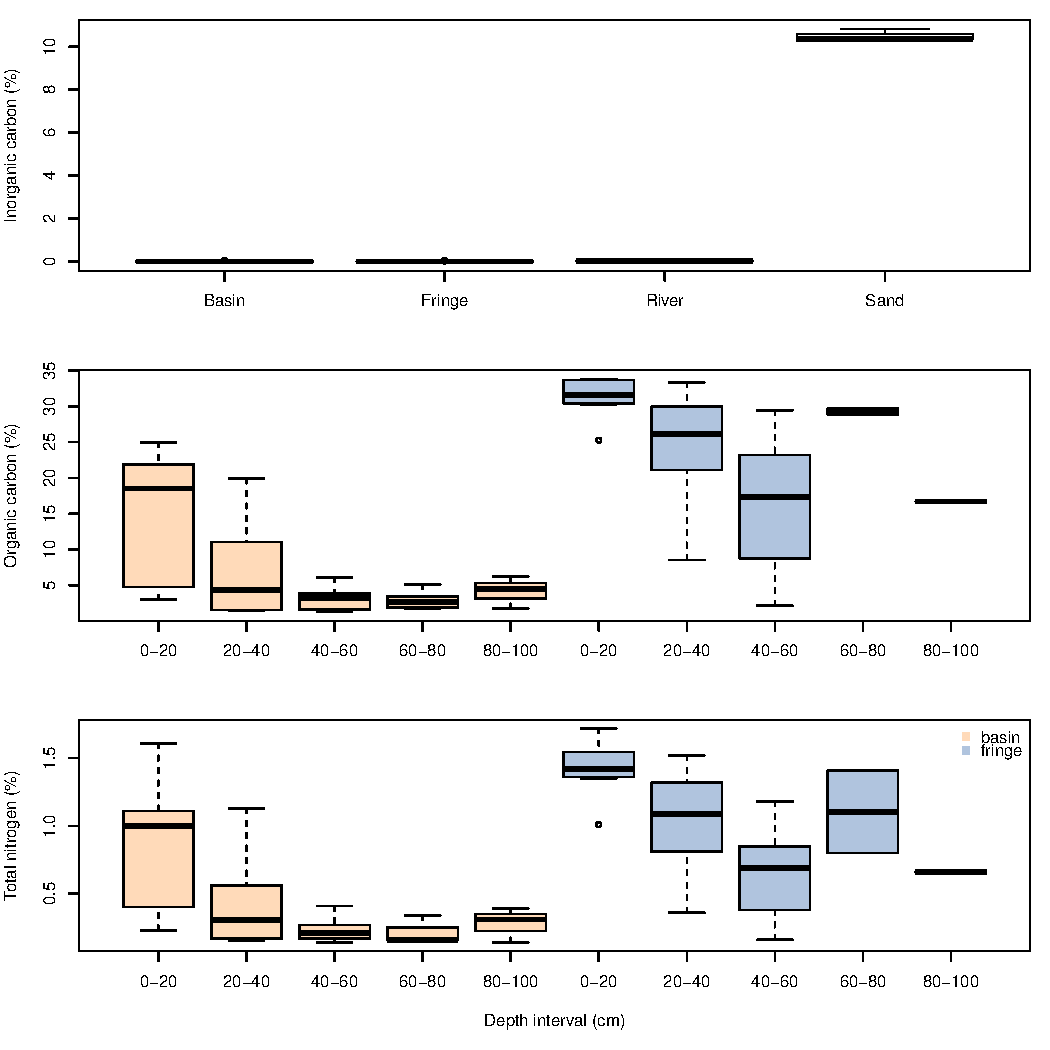
\includegraphics[width=12cm]{Figures/Fig2.pdf}
% figure caption is below the figure
\caption{Observed values of percent inorganic carbon (\%IC) for both mangrove types and end members; and percent organic carbon (\%OC) and percent nitrogen (\%TN) by sampling depth aggregated across plots. }
\label{fig:2}       % Give a unique label
\end{figure}

% Fig 3
\begin{figure}[H]
%\centering
%  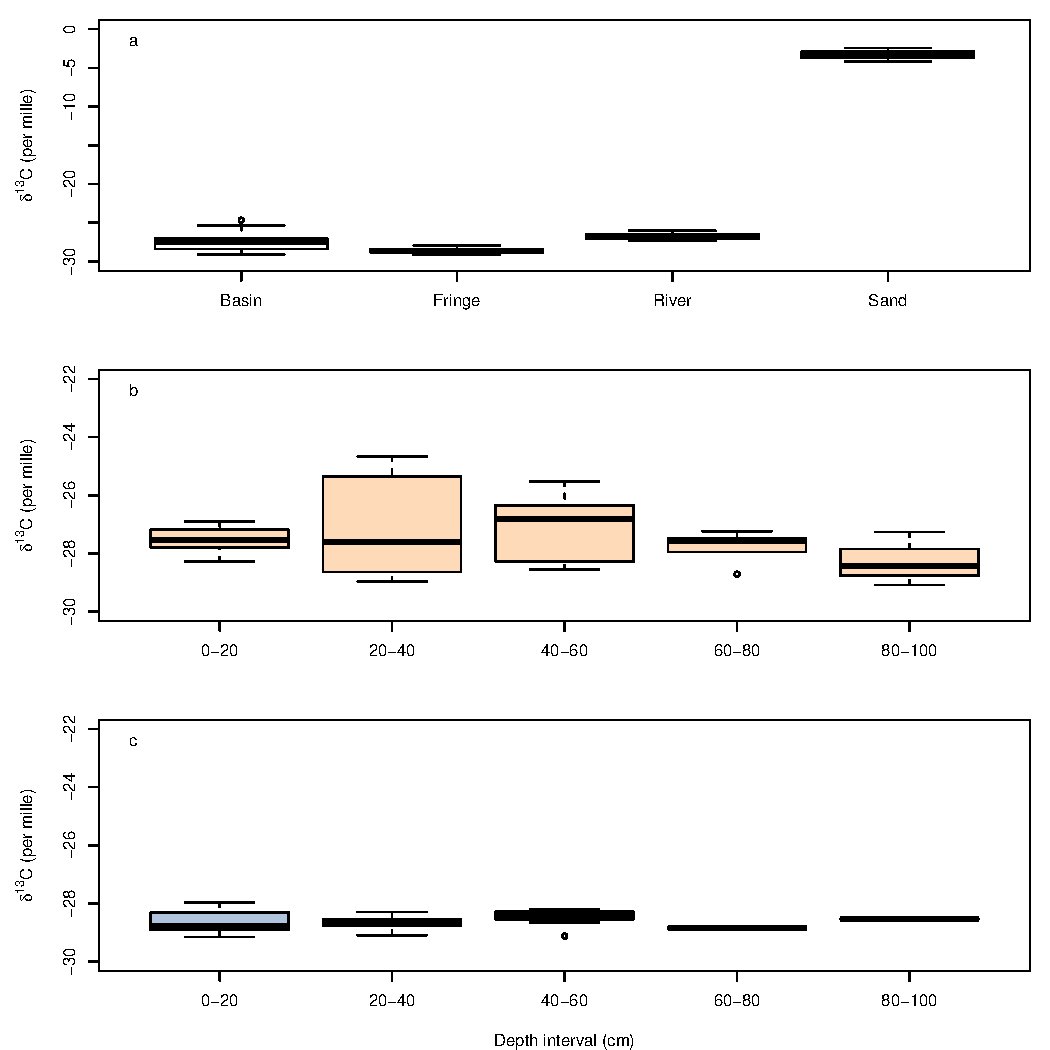
\includegraphics[width=12cm]{Figures/Fig3.pdf}
% figure caption is below the figure
\caption{Measured $\updelta^{13}$C in a) mangrove types and end members, b) basin mangroves by depth, and c) fringe mangroves by depth. }
\label{fig:3}       % Give a unique label
\end{figure}

% Fig 4
\begin{figure}[H]
%\centering
%  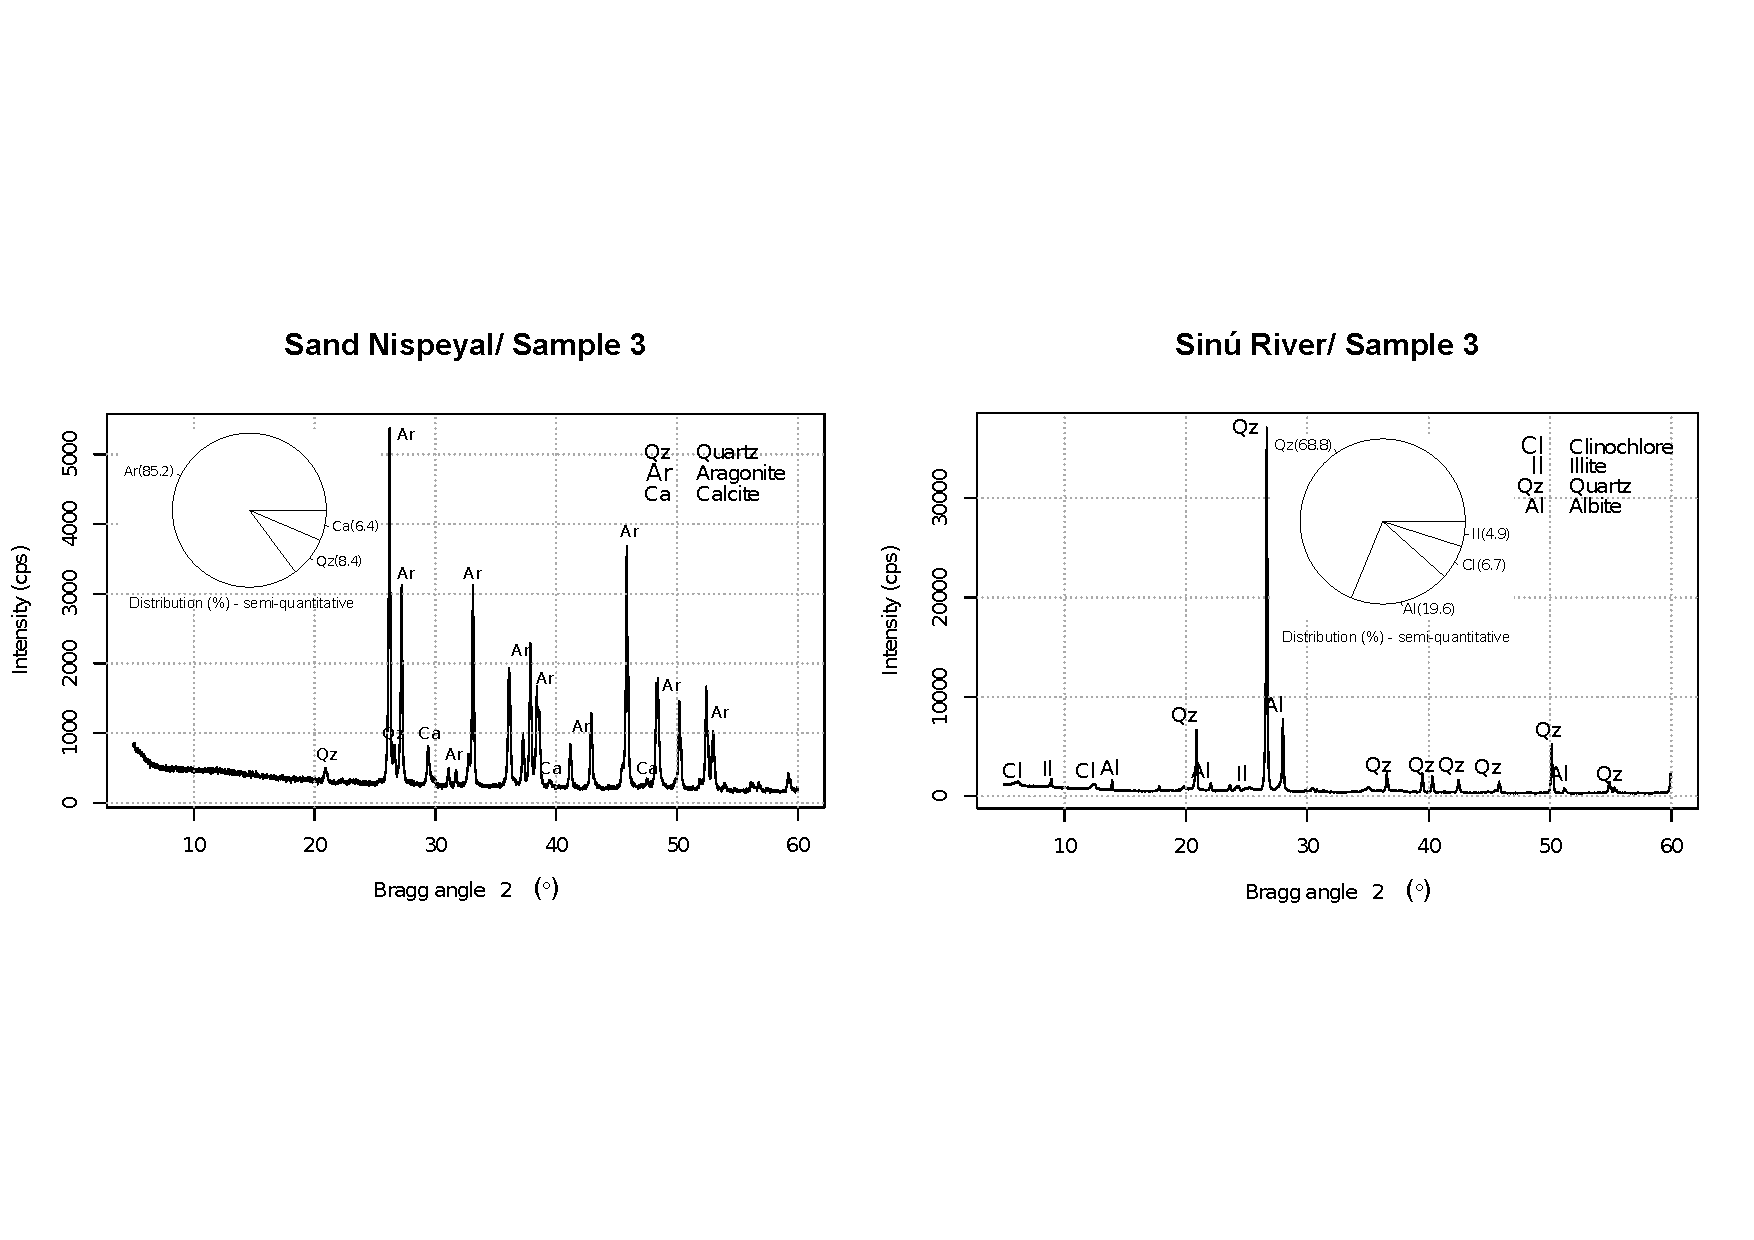
\includegraphics[width=12cm]{Figures/EndMembers.pdf}
% figure caption is below the figure
\caption{Two exemplary XRD patterns ($\uplambda$ = 1.5406 \AA) of both measured end-members: Nisperal beach and Sin\'{u} river; figures also include semi-quantitative distribution of detected minerals}
\label{fig:4}       % Give a unique label
\end{figure}

% Fig 5
\begin{figure}[H]
%\centering
%  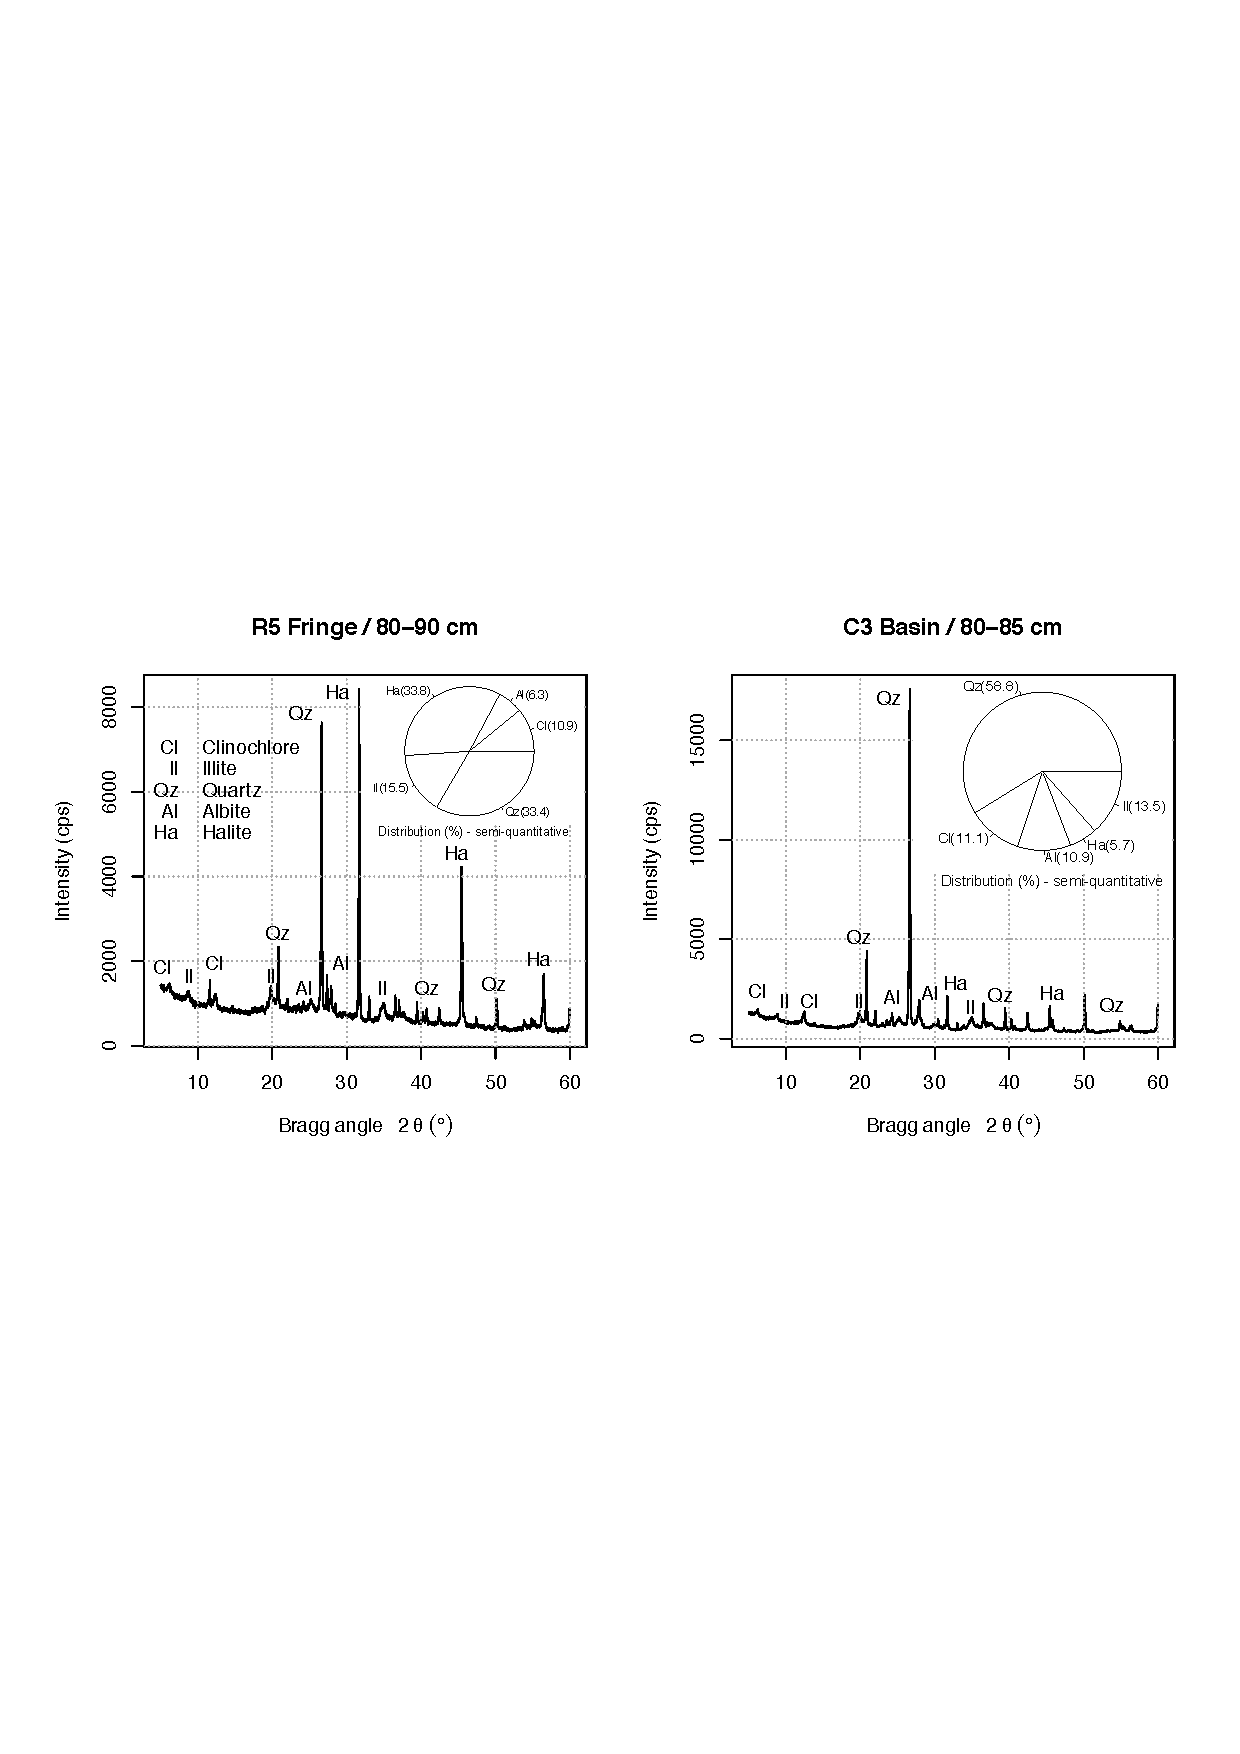
\includegraphics[width=12cm]{Figures/R5_C3.pdf}
% figure caption is below the figure
\caption{Two exemplary XRD patterns ($\uplambda$ = 1.5406 \AA) for the fringe (left) and basin (right) mangrove soils; figures also include semi-quantitative distribution of detected minerals}
\label{fig:5}       % Give a unique label
\end{figure}

% Fig 6
\begin{figure}[H]
%\centering
%  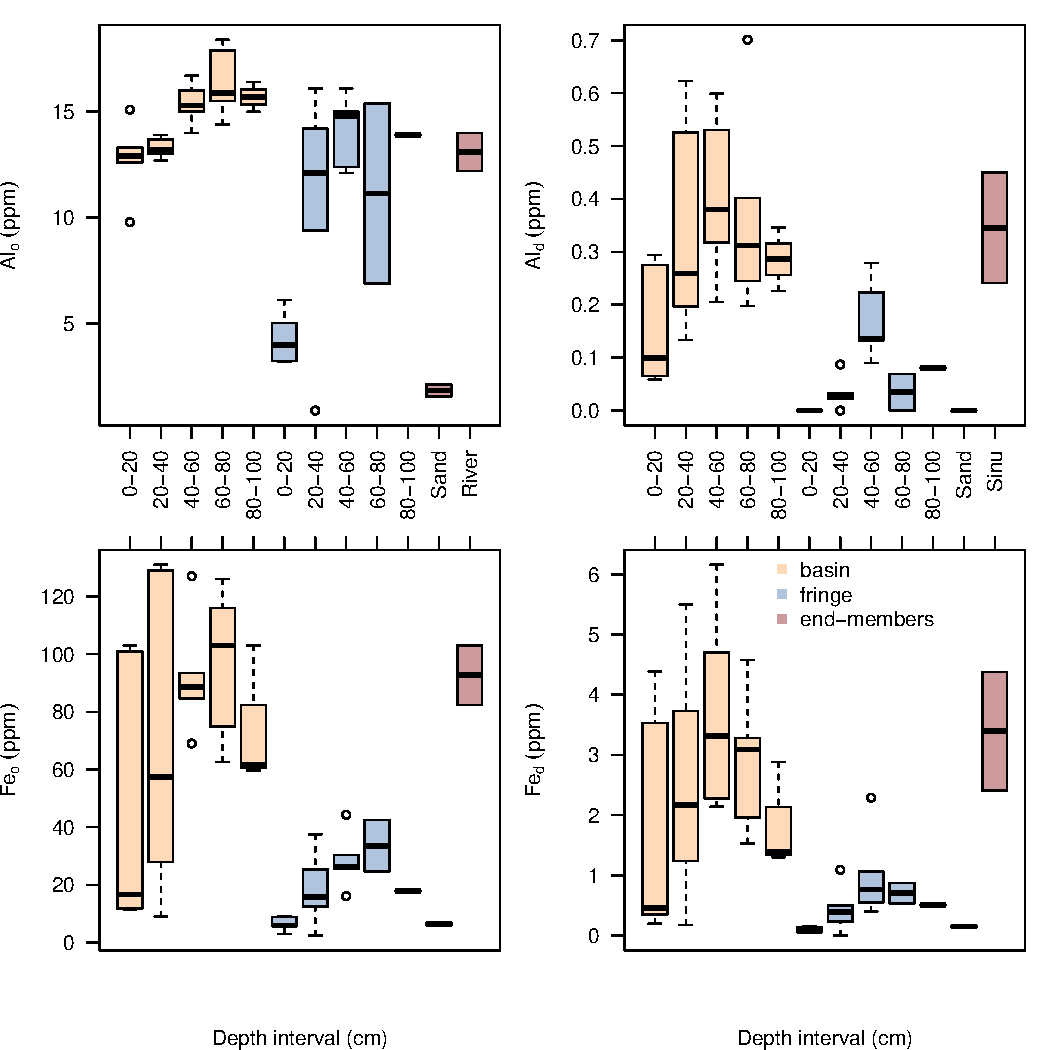
\includegraphics[width=12cm]{Figures/Fig6.pdf}
% figure caption is below the figure
\caption{Oxalate (o)- and dithionite (d) extracted metal oxides for each mangrove type and soil depth.}
\label{fig:6}       % Give a unique label
\end{figure}

\clearpage

\section*{Tables}

%Table 1
\begin{table}[H]
% table caption is above the table
\caption{Percent organic carbon, bulk density and total organic carbon by mangrove type and soil depth. Values in parentheses indicate standard deviation}
\label{tab:1}       % Give a unique label
% For LaTeX tables use
\begin{tabular}{lllll}
\hline\noalign{\smallskip}
Mangrove type & Depth [cm] & OC [\%]  & Bulk density [g/cm$^3$] & TOC [MgC/ha]\\
\noalign{\smallskip}\hline\noalign{\smallskip}
Basin & 0-20 & 14.63 (10.09) & 1.01 (0.06) & 295.61 (203.77)\\
 & 20-40 & 7.12 (7.19) & 1.25 (0.10) & 161.99 (147.07)\\
 & 40-60 & 3.22 (1.93) & 1.06 (0.19) & 68.35 (40.95)\\
 & 60-80 & 2.96 (1.39) & 1.10 (0.16) & 65.21 (30.58)\\
 & 80-100 & 4.15 (2.24) & 0.84 (0.08) & 69.78 (37.60)\\
\noalign{\smallskip}\hline\noalign{\smallskip}
Fringe & 0-20 & 31.32 (2.82) & 0.16 (0.01) & 100.24 (9.03)\\
 & 20-40 & 23.61 (8.70) & 0.13 (0.02) & 62.79 (22.56)\\
 & 40-60 & 16.12 (10.92) & 0.16 (0.05) & 51.57 (34.94)\\
 & 60-80 & 29.29 (0.55) & 0.18 (0.01) & 105.44 (1.99)\\
\noalign{\smallskip}\hline
\end{tabular}
\end{table}

% Table 2
\begin{table}[H]
% table caption is above the table
\caption{General mineralogical composition of sediments in Cispat\'{a} Bay as measured by XRD analyses.}
\label{tab:2}       % Give a unique label
% For LaTeX tables use
\begin{tabular}{lll}
\hline\noalign{\smallskip}
Class & Mineral  & Formula\\
\noalign{\smallskip}\hline\noalign{\smallskip}
Silicates & Clinochlore & (Mg,Fe$^{2+}$)$_5$Al(Si$_3$Al)O$_{10}$(OH)$_8$\\
& Illite & (K,H$_3$O)Al$_2$(Si$_3$Al)O$_{10}$(H$_2$O,OH)$_2$\\
& Albite & NaAlSi$_3$O$_8$\\
\noalign{\smallskip}\hline\noalign{\smallskip}
Oxides/hydrox. & Quartz & SiO$_2$\\
\noalign{\smallskip}\hline\noalign{\smallskip}
Carbonates & Aragonite & CaCO$_3$\\
& Calcite & CaCO$_3$\\
\noalign{\smallskip}\hline\noalign{\smallskip}
Halides & Halite & NaCl\\
\noalign{\smallskip}\hline
\end{tabular}
\end{table}



% BibTeX users please use one of
\bibliographystyle{spbasic}   % basic style, author-year citations
\bibliography{Reference}

   %\bibliographystyle{spmpsci}      % mathematics and physical sciences
%\bibliographystyle{spphys}       % APS-like style for physics
%\bibliography{}   % name your BibTeX data base

% Non-BibTeX users please use

%
% and use \bibitem to create references. Consult the Instructions
% for authors for reference list style.
%
%\bibitem{RefJ}
% Format for Journal Reference
%Author, Article title, Journal, Volume, page numbers (year)
% Format for books
%\bibitem{RefB}
%Author, Book title, page numbers. Publisher, place (year)
% etc
%\end{thebibliography}

\end{document}
% end of file template.tex

